\documentclass[12pt]{article}
\usepackage{graphicx} % Required for inserting images
\usepackage[a4paper, total={6in, 10in}]{geometry}
\usepackage{datetime, xcolor, tcolorbox, chngcntr, subcaption, float}
\usepackage{amsthm, thmtools, amsfonts, mathtools, amssymb, amsmath}

\counterwithin{figure}{section}

\tcbuselibrary{theorems}

\usepackage{tikz, scalerel, pict2e, tkz-euclide, pgfplots}

\usetikzlibrary{calc, patterns, arrows.meta, shadows, external}
\pgfplotsset{compat=newest}
\usepgfplotslibrary{statistics, fillbetween}


\newdateformat{monthyeardate}{\monthname[\THEMONTH] \THEYEAR}

\newtheorem{theorem}{Theorem}[section]
\newtheorem{corollary}{Corollary}[theorem]
\newtheorem{lemma}[theorem]{Lemma}
\newtheorem{axiom}{Axiom}
\newtheorem{proposition}{Proposition}[section]
%\newtheorem{definition}{Definition}[section]
\theoremstyle{remark}
\newtheorem*{remark}{Remark}
\newtheorem*{notation}{Notation}

\definecolor{box-head}{rgb}{0, 0.435, 0.510}
\definecolor{box-body}{rgb}{0.506, 0.718, 0.757}

\newtcolorbox{important}[1][]{colframe=box-head, colback=box-body!28!, title=#1, fonttitle=\bfseries, before skip = 10pt}

\declaretheoremstyle[
    spaceabove=5pt, 
    spacebelow=6pt, 
    headfont=\normalfont\bfseries, 
    bodyfont = \normalfont,
    headpunct={:}]{definitionstyle} 
\declaretheorem[name={Definition}, style=definitionstyle, numberwithin=section]{definition}
\declaretheorem[name={Example}, style=definitionstyle, numberwithin=section]{example}

\let\oldvec = \vec
\renewcommand{\vec}[1]{\oldvec{\mathbf{#1}}}


\numberwithin{equation}{section}


\title{Linear Algebra}
\author{Riddhiman}
\date{\monthyeardate\today}

\begin{document}

\maketitle

\section{Preface}%
\label{sec:Preface}
Self study Linear Algebra notes. Source is \textit{Vector Calculus, Linear Algebra, and Differential Geometry} by John and Barbara Hubbard. These notes will start from Section 1.3. Notes for Sections 1.1 and 1.2 will be added later.

\section{Matrix Multiplication as Linear Transformation}%
\label{sec:Matrix Multiplication as Linear Transformation}

\begin{definition}[Linear transformation from $ \mathbb{R}^n $ to $ \mathbb{R}^m $]  
	A \textit{linear transformation} $ T : \mathbb{R}^{n} \rightarrow \mathbb{R}^{m} $ is a mapping such that for all scalars $ a $ and for all $ \vec{v}, \vec{w} \in \mathbb{R}^{n} $,
	\begin{equation}
		T(\vec{v} + \vec{w}) = T(\vec{v}) + T(\vec{w}) \text{ and } T(a\vec{v}) = aT(\vec{v})
	\end{equation}	
\end{definition}

This above was the definition of a linear transformation. The following theorem will relate matrices to linear transformation. 

\begin{important}[Theorem 2.1 (Matrices and linear transformation)]
	\begin{enumerate}
		\item Any $ m \times n $ matrix $ A $ defines a linear transformation $ T : \mathbb{R}^n \rightarrow \mathbb{R}^m $ is given by matrix multiplication: 
			\begin{equation}
				T(\vec{v}) = A \vec{v}.	
			\end{equation}
		\item Every linear transformation $ T : \mathbb{R}^n \rightarrow \mathbb{R}^m $ is given by multiplication by the $ m \times n $ matrix $ [T] $:
			\begin{equation}
				T(\vec{v}) = [T]\vec{v}, 
			\end{equation}
			where the $ i^{\text{th}} $ column of $ [T] $ is $ T(\vec{e}_{i}) $.
	\end{enumerate}
\end{important}

\begin{proof}[Proof to part 2 of Theorem 2.1] 
	Given that our domain is $ \mathbb{R}^n $ we can write any vector $ \vec{v} \in \mathbb{R}^n $ as \[\vec{v} = u_{1}\vec{e}_{1} + u_{2}\vec{e}_{2} + \ldots + u_{n}\vec{e}_{n} = %
	\sum^{n}_{i=1} u_{i}\vec{e}_{i} \]
	Thus, 
	\begin{align*}
		T(\vec{v}) &= T\left(\sum^{n}_{i=1} u_{i}\vec{e}_{i}\right) \\ 
			   &= \sum^{n}_{i=1} u_{i}T(\vec{e}_{i}) 
	\end{align*}
	Also note that since every $ i^{\text{th}} $ column of $ [T] $ is $ T(\vec{e}_{i}) $. When $ [T] $ is multiplied by $ \vec{v} $, the $ i^{\text{th}} $ of the resultant column vector can be denoted as $ u_{1}T(\vec{e}_{1}) + \ldots + u_{n}T(\vec{e}_{n}) $ which is just $ T(\vec{v}) $. 
\end{proof}

\subsection{Finding the matrix of a linear transformation}%
\label{sub:Finding the matrix of a linear transformation}

By Theorem 2.1 is it clear that to find the matrix say $ [T] $ associated with the linear transformation $ T $ we have to find what $ T $ does to the basis vectors $ \vec{e}_{i} $. \par

For example, consider a straight line passing through the origin of $ \mathbb{R}^2 $. Also consider two arbitrary vectors $ \textcolor{red}{\vec{a}} $ and $ \textcolor{blue}{\vec{b}} $. We wish to find the resultant vectors when $ \textcolor{red}{\vec{a}} $ and $ \textcolor{blue}{\vec{b}} $ are reflected about the line. Using the figure below it is easy to see that the act of reflecting vectors about a straight line passing through the origin is a linear transformation. Let this transformation be called $ T $. 

\begin{figure}[htp]
    \centering
        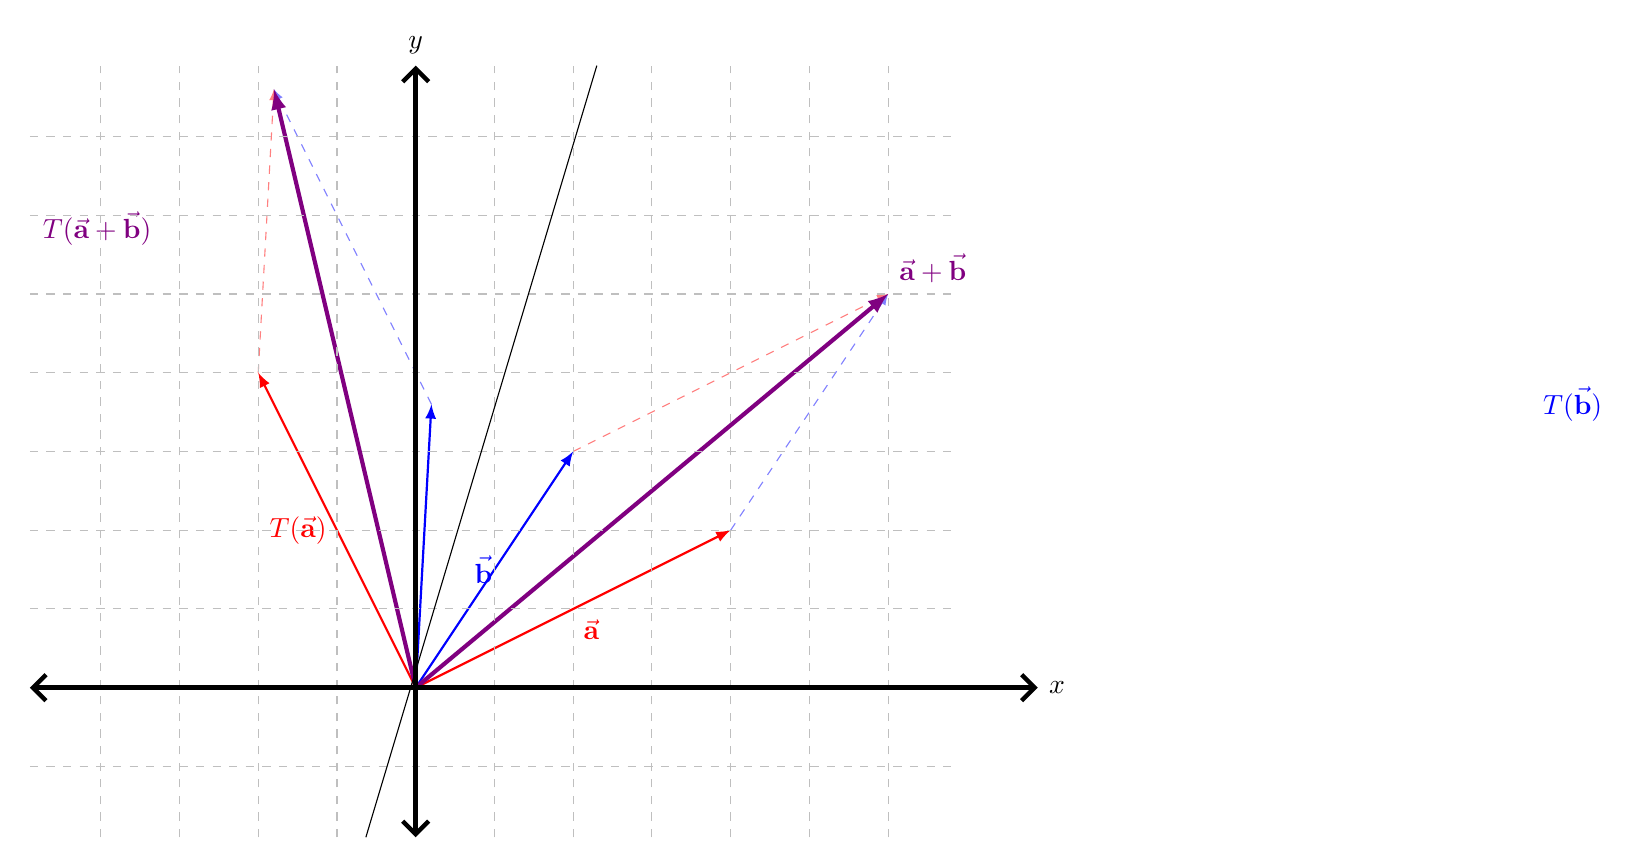
\begin{tikzpicture}[scale=1]
	% vectors
	\draw[thick, -latex, red] (0, 0) -- (4, 2) node[midway, below right] {$ \vec{a} $};
	\draw[-latex, blue!50, dashed] (4, 2) -- (6, 5);
	\draw[thick, -latex, blue] (0, 0) -- (2, 3) node[midway, above=8pt, left=-3pt] {$ \vec{b} $};
	\draw[-latex, red!50, dashed] (2, 3) -- (6, 5);

	% vectors added
	\draw[line width=1.5pt, -latex, violet] (0, 0) -- (6, 5) node[above right] {$ \vec{a} + \vec{b} $};

	% reflected vectors
	\draw[thick, -latex, red] (0, 0) -- (-2, 4) node[midway, below, left] {$ T(\vec{a}) $};
	\draw[thick, -latex, blue] (0, 0) -- (0.2, 3.6) node[above=10, left = -15] {$ T(\vec{b}) $};
	\draw[-latex, blue!50, dashed] (0.2, 3.6) -- (-1.8, 7.6);
	\draw[-latex, red!50, dashed] (-2, 4) -- (-1.8, 7.6);

	% reflected vectors added
	\draw[line width=1.5pt, -latex, violet] (0, 0) -- (-1.8, 7.6) node[below left=2] {$ T(\vec{a} + \vec{b}) $};


	% axes and grid
	\draw[help lines, color=gray!50, dashed] (-4.9, -1.9) grid (6.9,7.9);
	\draw[ultra thick, Straight Barb-Straight Barb] (-4.9, 0) -- (7.9, 0) node[right] {$ x $};
	\draw[ultra thick, Straight Barb-Straight Barb] (0, -1.9) -- (0, 7.9) node[above] {$ y $};
	\draw[] (-0.633,-1.9) -- (2.3, 7.9);
	\end{tikzpicture}
	\caption{Reflection is linear}

\end{figure}

Recall that the first column of $ [T] $ is $ T\left( \begin{bmatrix} 
							1 \\
							0
						      \end{bmatrix} \right) $,
and thus the second column is $ T \left(
				\begin{bmatrix}
					0 \\
					1
				\end{bmatrix}
				\right) $. 
Let the line make an angle $ \theta $ with the x-axis. Then the matrix comes out to be
\[ 
	[T] = 
	\begin{bmatrix}
		\cos{2\theta} &  \phantom{-}\sin{2\theta} \\
		\sin{2\theta} & -\cos{2\theta}
	\end{bmatrix}
\]

Now just multiply this matrix by any vector to get the reflected vector. This is how matrices behave -- they encode linear transformations. \par

Another example of a linear transformation is the projection matrix. This matrix projects given vectors onto a certain line passing through the origin. If said line is making an angle $ \theta $ with the x-axis then the matrix is 
\[  
	\begin{bmatrix}
		\cos^{2}{\theta} & \sin{\theta}\cos{\theta} \\
		\sin{\theta}\cos{\theta} & \sin^{2}{\theta}
	\end{bmatrix}
\]

In both the cases above, how the where the basis vectors land after applying the transformation was found by basic trigonometry. 

\subsection{Geometry interpretation of linear transformation}%
\label{sub:Geometry interpretation of linear transformation}

A linear transformation may be applied to entire subsets of $ \mathbb{R}^n $ instead of just individual vectors. Here are some transformations, their matrix representations, and how each point in $ \mathbb{R}^n $ behaves when transformed. 

\begin{example}[Identity transformation]
	The identity transformation : $ \mathbb{R}^n \rightarrow \mathbb{R}^n $ is represented by $ I_{n} $. Applying this transformation to a subset of $ \mathbb{R}^n $ leaves it unchanged.  
\end{example}

\begin{example}[Scaling transformation]
    This transformation $ T $ enlarges everything by a factor of $ a $ and is given by % 
    $ \begin{bmatrix} a & 0 \\ 0 & a \end{bmatrix} $.   
\end{example}

\begin{example}[Stretching transformation]
	These transformations are of the form $ \begin{bmatrix} 2 & 0 \\ 0 & 1 \end{bmatrix} $. It will stretch the unit square into a rectangle. 
\end{example}

\begin{example}[Rotation transformation]
	This is a transformation $ R $ which rotates the subset by an angle $ \theta $ in the counterclockwise around the origin. This is given by 
	\[
	[R] = 
	 \begin{bmatrix}
		 \cos{\theta} & -\sin{\theta} \\
		 \sin{\theta} & \phantom{-}\cos{\theta}
	 \end{bmatrix}
	\]
\end{example}

\begin{figure}[htbp]
	\centering
	\begin{subfigure}[]{0.4\linewidth}
	% scaling transformation
	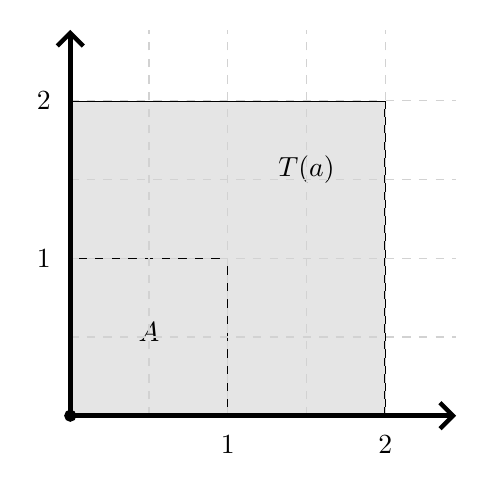
\begin{tikzpicture}
		% transformed square
		\draw[fill=gray!20, line width=0.1pt] (0, 0) rectangle (4, 4);
		\draw[line width=0.7pt, dashed] (4, 0) -- (4, 4);
		\draw[line width=0.7pt, dashed] (0, 4) -- (4, 4);
		\node[label=$ T(a) $] at (3, 2.7) {};

		% unit square
		\draw[fill=gray!20] (0, 0) rectangle (2, 2);
		\draw[line width=0.5pt] (2, 0) -- (2, 2);
		\draw[line width=0.5pt] (0, 2) -- (2, 2);
		\node[label=$ A $] at (1, 0.7) {};


		% axes and grid
		\draw[help lines, color=gray!35, dashed] (0, 0) grid (4.9,4.9);
		\draw[ultra thick, -Straight Barb] (0, 0) -- (4.9, 0);
		\draw[ultra thick, -Straight Barb] (0, 0) -- (0, 4.9);
		\filldraw[black] (0, 0) circle (2pt);
		\node[label=below:{$ 1 $}] at (2, 0) {};
		\node[label=left:{$ 1 $}] at (0, 2) {};
		\node[label=left:{$ 2 $}] at (0, 4) {};
		\node[label=below:{$ 2 $}] at (4, 0) {};
	\end{tikzpicture}%
	\caption{The scaling transformation given by $ \begin{bmatrix} 2&0\\0&2 \end{bmatrix}$ turns the unit square into the square with side length 2}.
	\end{subfigure}\hspace*{\fill}%
	\begin{subfigure}[]{0.4\linewidth}
    % scaling transformation
	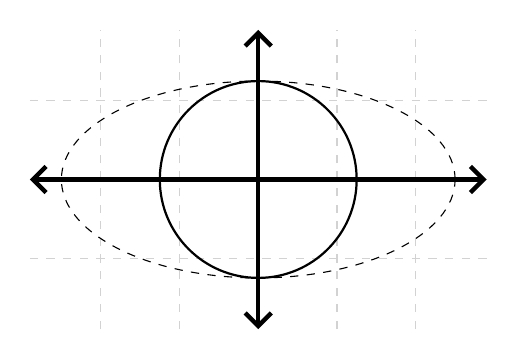
\begin{tikzpicture}
		% axes and grid
		\draw[help lines, color=gray!35, dashed] (-2.9, -1.9) grid (2.9,1.9);
		\draw[ultra thick, Straight Barb-Straight Barb] (-2.9, 0) -- (2.9, 0);
		\draw[ultra thick, Straight Barb-Straight Barb] (0, -1.9) -- (0, 1.9);

		% unit circle
		\node[circle, draw, minimum size = 2.5cm, thick] (c) at (0, 0) {};
		
		% transformed circle
		\draw[dashed] (0, 0) ellipse (2.5cm and 1.25cm);
		\end{tikzpicture}
	\caption{The linear transformation given by $ \begin{bmatrix} 2&0\\0&1 \end{bmatrix} $ stretches the unit circle into an ellipse}

	\end{subfigure}

\end{figure}

\begin{important}[Theorem 2.2 (Composition corresponds to matrix multiplication)]
	Suppose $ S : \mathbb{R}^n \rightarrow \mathbb{R}^m $ and $ T : \mathbb{R}^m \rightarrow \mathbb{R}^l $ are linear transformations given by the matrices $ [S] $ and $ [T] $ respectively. Then the $ [T \circ S] $ is linear and 
	\begin{equation}
		[T \circ S] = [T][S]
	\end{equation}
	
    
\end{important}

\begin{proof}
    First we will prove that $ T \circ S $ is indeed a linear transformation. Hence, consider the following 
    \begin{align*}
	    ( T \circ S )(a \vec{v} + b \vec{w}) &= T(S(a \vec{v} + b \vec{w})) = T(a S(\vec{v}) + b S(\vec{w})) \\ 
						 &= T(a S(\vec{v})) + T(b S(\vec{w})) \\ 
						 &= a T(S(\vec{v})) + T(S(\vec{w})) \\ 
						 &= a(T \circ S)(\vec{v}) + b(T \circ S)(\vec{w}). 
    \end{align*}
    This shows that $ T \circ S $ is a linear transformation has a corresponding matrix $ [T \circ S] $. Now we have to prove Equation 2.4. For this we will use the following two facts: 
    \begin{enumerate}
	\item $ A \vec{e}_{i} $ is the $ i^{\text{th}} $ column of $ A $.
	\item The $ i^{\text{th}} $ column of $ AB $ is $ A \vec{b}_{i} $ where $ \vec{b}_{i} $ is the $ i^{\text{th}} $ column of $ B $.
    \end{enumerate}
    Now, 
    \begin{equation}
	    [T \circ S] \vec{e}_{i} = (T \circ S)(\vec{e}_{i}) = T(S(\vec{e}_{i})) %
	    = T([S]\vec{e}_{i}) = [T]([S]\vec{e}_{i}).
    \end{equation}
    Notice that by fact (1), $ [T \circ S]\vec{e}_{i} $ is the $ i^{\text{th}} $ column of $ [T \circ S] $ and that $ [S]\vec{e}_{i} $ is the $ i^{\text{th}} $ column of $ [S] $, and thus by fact (2), $ [T]([S]\vec{e}_{i}) $ becomes the $ i^{\text{th}} $ column of $ [T][S] $. Since the columns of $ [T \circ S] $ and $ [T][S] $ are equivalent, they are the same matrix, which proves Equation 2.4.
\end{proof}

Given below is an example desmostrating composition of linear transformations. 

\begin{figure}[htp]
    % scaling transformation
	\centering
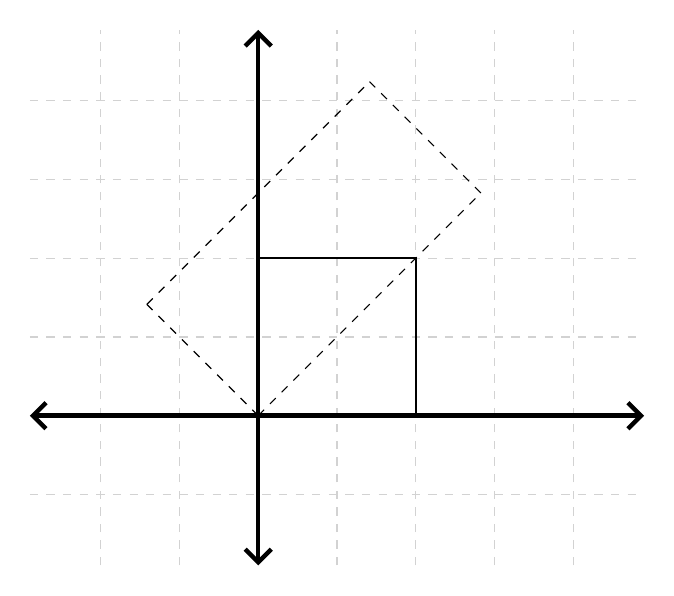
\begin{tikzpicture}
	% axes and grid
	\draw[help lines, color=gray!35, dashed] (-2.9, -1.9) grid (4.9,4.9);
	\draw[ultra thick, Straight Barb-Straight Barb] (-2.9, 0) -- (4.9, 0);
	\draw[ultra thick, Straight Barb-Straight Barb] (0, -1.9) -- (0, 4.9);

	% unit square
	\draw[thick] (0, 0) rectangle (2, 2);

	% stretched and rotated square
	\draw[dashed] (0, 0) -- (2.82842712, 2.82842712); % i hat
	\draw[dashed] (0, 0) -- (-1.41421356237, 1.41421356237); % j hat
	\draw[dashed] (2.82842712, 2.82842712) -- (1.41421356237, 4.24264068712);
	\draw[dashed] (-1.41421356237, 1.41421356237) -- (1.41421356237, 4.24264068712); 
\end{tikzpicture}
\caption{Result of applying $ \begin{bmatrix} % 
		\cos{\frac{\pi}{4}} & -\sin{\frac{\pi}{4}} \\ 
		\sin{\frac{\pi}{4}} & \phantom{-}\cos{\frac{\pi}{4}} %
				\end{bmatrix} $ %
		$	\begin{bmatrix}
				2 & 0 \\
				0 & 1 %
			\end{bmatrix} $ %
			} to the unit square. 
\end{figure}


\end{document}

